
%(BEGIN_QUESTION)
% Copyright 2015, Tony R. Kuphaldt, released under the Creative Commons Attribution License (v 1.0)
% This means you may do almost anything with this work of mine, so long as you give me proper credit

In this process, sulfur-laden water is ``stripped'' of sulfur compounds by the addition of hot steam:

$$\includegraphics[width=15.5cm]{i0007rx01.eps}$$

Operators note that changes made to the setpoint value of FIC-27 have the undesired effects of pushing the process variables of TIC-21 and LIC-12 off of their respective setpoints.  Modify the control strategy(ies) shown here to include {\it feedforward} as a solution to these observed load changes.

\underbar{file i02884}
%(END_QUESTION)





%(BEGIN_ANSWER)

First, we must clearly understand what the loading effects will be (i.e. which direction the load changes will affect TIC-21 and LIC-12).  Performing a thought experiment where we suddenly increase the amount of cold liquid feed into the stripper vessel (C-7), we see this will {\it decrease} temperature within that vessel which reduces the need for cooling water controlled by TIC-21 and drive the temperature (process variable for TIC-21) under setpoint.  Increasing sour water flow into the vessel will also {\it increase} the level of liquid accumulated at the bottom which will demand an increased flow rate of stripped water leaving the vessel and heading toward the water treatment process, driving the liquid level (process variable for LIC-12) above setpoint.

\vskip 10pt

The purpose of feedforward control is to preemptively move a final control element in response to a change in load, such that the loading effects will be canceled and the feedback control system need not correct for it.  In this case, we will need to take the flow signal output by FT-27 and use that flow signal to negatively bias control valve TV-21 (i.e. reducing cooling water flow as the cold feed flow increases) and positively bias control valve LV-12 (i.e. increasing stripped water flow as feed flow increases).

\vskip 10pt

Perhaps the most significant obstacle to implementing feedforward control in these two loops is the fact that both feedback control loops are entirely pneumatic, while FT-27 outputs an electronic signal.  The ``summing'' functions necessary to add the feedforward signal to the control valve signals (TV-21 and LV-12) will need to be pneumatic summer instruments, and the electronic feedforward signal from FT-27 will need to enter an I/P converter to change it to a pneumatic signal.  An alternative plan, of course, would be to upgrade both controllers (TIC-21 and LIC-12) to electronic instead of pneumatic in order to make the feedforward strategy much easier to implement.

This diagram shows what the feedforward strategy would look like, with the process vessels and piping removed for simplicity:

$$\includegraphics[width=15.5cm]{i02884x01.eps}$$


%(END_ANSWER)





%(BEGIN_NOTES)


\vskip 20pt \vbox{\hrule \hbox{\strut \vrule{} {\bf Virtual Troubleshooting} \vrule} \hrule}

This question is a good candidate for a ``Virtual Troubleshooting'' exercise.  Presenting the diagram to students, you first imagine in your own mind a particular fault in the system.  Then, you present one or more symptoms of that fault (something noticeable by an operator or other user of the system).  Students then propose various diagnostic tests to perform on this system to identify the nature and location of the fault, as though they were technicians trying to troubleshoot the problem.  Your job is to tell them what the result(s) would be for each of the proposed diagnostic tests, documenting those results where all the students can see.

During and after the exercise, it is good to ask students follow-up questions such as:

\begin{itemize}
\item{} What does the result of the last diagnostic test tell you about the fault?
\item{} Suppose the results of the last diagnostic test were different.  What then would that result tell you about the fault?
\item{} Is the last diagnostic test the best one we could do?
\item{} What would be the ideal order of tests, to diagnose the problem in as few steps as possible?
\end{itemize}

%INDEX% Control, strategies: feedforward 
%INDEX% Process: sour water stripping tower (realistic P&ID shown)

%(END_NOTES)

